autenticação api dados RPD

De modo a proceder à autenticação de pedidos à \gls{api}, irá ser implementado um sistema baseado em \emph{JSON Web Tokens}.

Esta implementação seguirá as normas propostas pelo \emph{"OAuth 2.0 Authorization Framework: Bearer Token Usage"}\cite{rfc6750}, utilizando para o efeito um header HTTP do tipo \emph{Authorization}, com esquema de autenticação \emph{Bearer}\footnote{Mais informação em \url{https://www.iana.org/assignments/http-authschemes/http-authschemes.xhtml}}.

\begin{figure}[h]
    \centering
    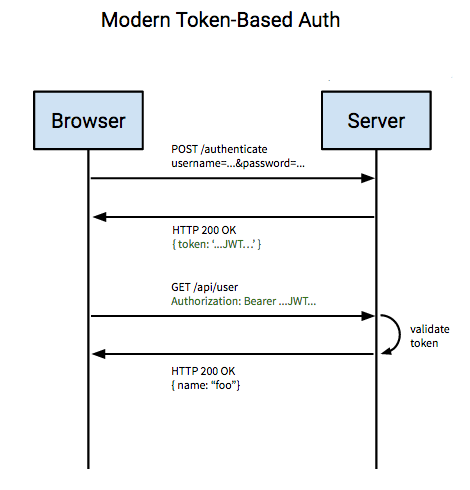
\includegraphics[width=0.75\textwidth]{img/jwt/diagramafluxoJWT.png}
    \caption{Diagrama correspondente à autenticação baseda em tokens. \cite{jwtDiagram}}
\end{figure}

O sistema de autenticação a ser implementado seguirá o diagrama previamente descrito, ou seja:

\begin{enumerate}
    \item É realizada a autenticação de um elemento externo no nosso servidor.
    \item Caso a autenticação tenha sucesso, irá ser devolvido um \gls{jwt} que irá servir de \emph{API Key} para a autenticação de chamadas à mesma.
    \item Cada vez que é feita uma chamada à \gls{api}, o token presente no campo \emph{Authorization} irá ser validado.
    \item Caso este seja validado com sucesso, irá ser retornado o output da chamada à API solicitada.
\end{enumerate}

Outra possibilidade de implementação é descrita a seguir, onde no servidor 3 (neste caso, o servidor responsável por correr o projeto \gls{clav}), possui uma lista de \emph{API Key} válidas (neste caso, \gls{jwt}).

\begin{figure}[h]
    \centering
    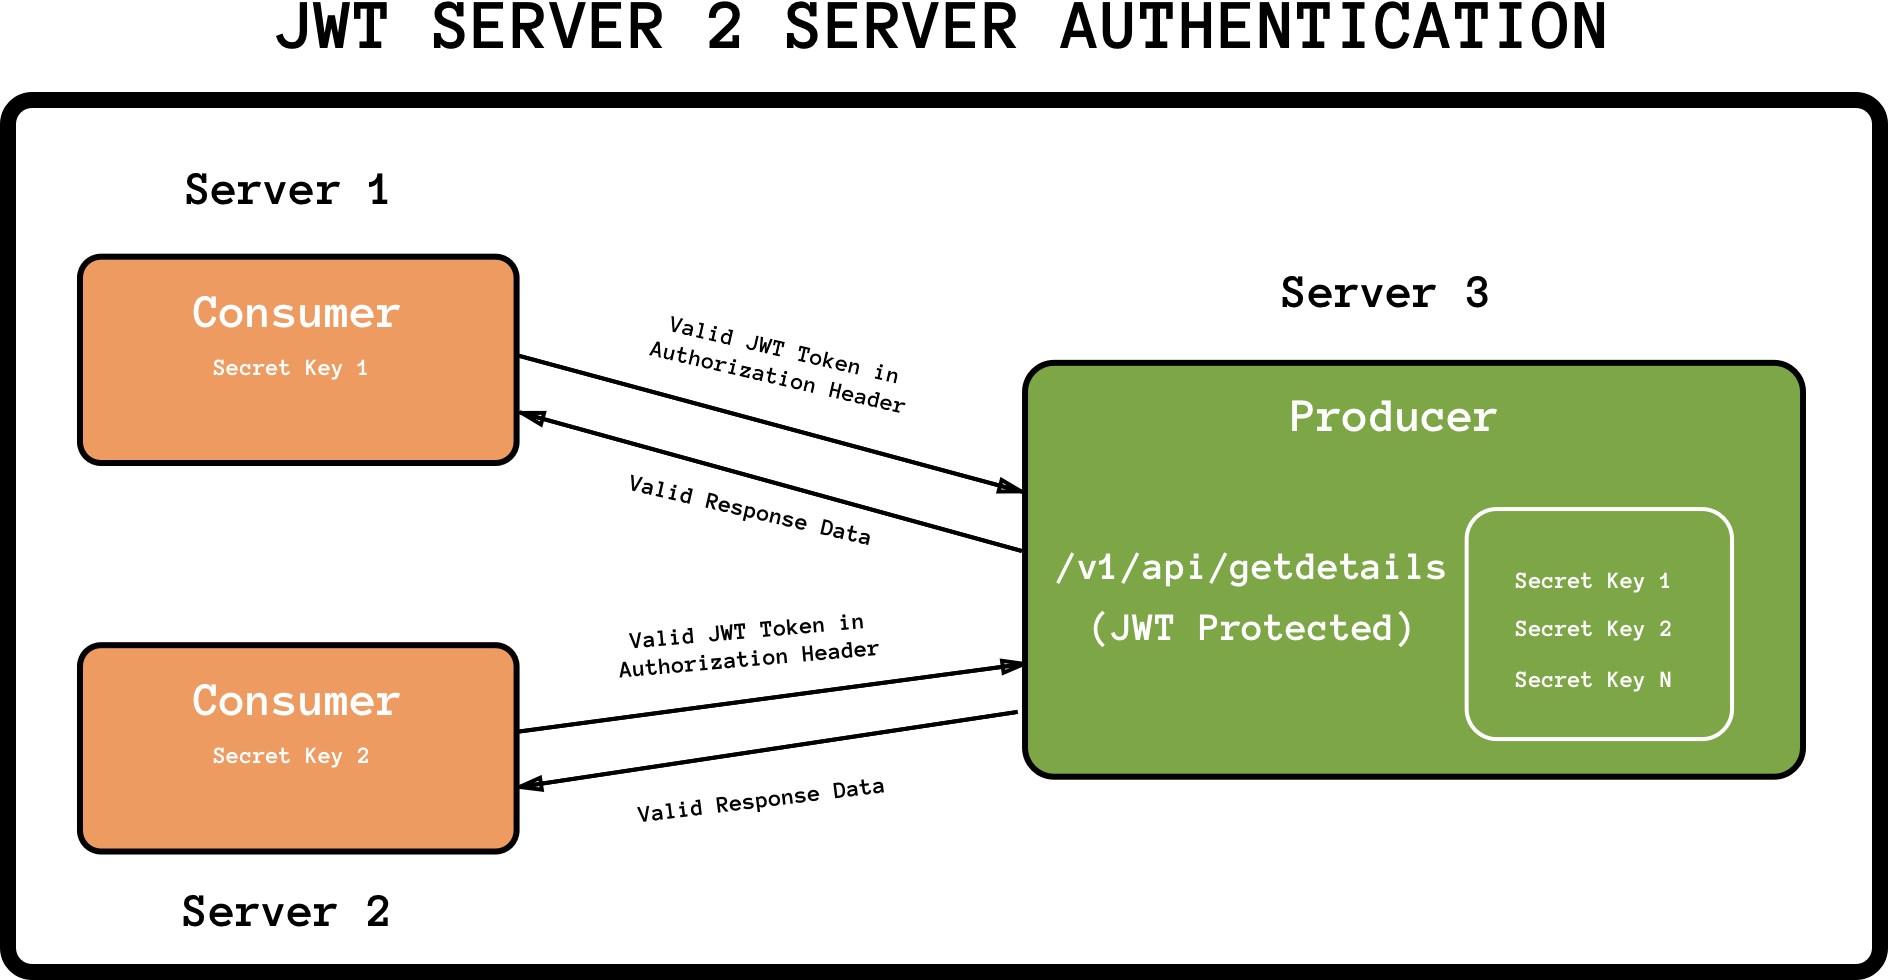
\includegraphics[width=\textwidth]{img/jwt/jwtAPI.png}
    \caption{Representação da utilização de \emph{JSON Web Token} para autenticação de pedidos à API. \cite{jwtAPI}}
\end{figure}

Cada vez que uma chamada à \gls{api} é feita, irá ser verificado se o \emph{token} dos utilizadores (representados por consumidores na imagem), está presente na lista de chaves pré validadas.